\documentclass[6pt, twocolumn]{article}

%%%%%%%%%%%%%%%%%%%%%%%%%%%%%%%%%%%%%%%%%%%%%%%%%%%%%%%%%%%%%%%%%%%%%%%%%%%
%
% Plantilla para un artículo en LaTeX en español.
%
%%%%%%%%%%%%%%%%%%%%%%%%%%%%%%%%%%%%%%%%%%%%%%%%%%%%%%%%%%%%%%%%%%%%%%%%%%%

% Qué tipo de documento estamos por comenzar:

% Esto es para que el LaTeX sepa que el texto está en español:
\usepackage[spanish]{babel}
\selectlanguage{spanish}
% Esto es para poder escribir acentos directamente:
\usepackage[utf8]{inputenc}
\usepackage[T1]{fontenc}



%% Asigna un tamaño a la hoja y los márgenes
\usepackage[a4paper,top=1cm,bottom=1.3cm,left=1.3cm,right=1.3cm,marginparwidth=1.3cm]{geometry}

%% Paquetes de la AMS
\usepackage{amsmath, amsthm, amsfonts}
%% Para añadir archivos con extensión pdf, jpg, png or tif
\usepackage{graphicx}
\usepackage[colorinlistoftodos]{todonotes}
\usepackage[colorlinks=true, allcolors=blue]{hyperref}

%% Primero escribimos el título
\title{Modelo para la Predicción de la Supervivencia de Pacientes con Carcinoma Hepatocelular (HCC)}
\footnotesize
\author{José Emanuel Rodríguez Fitta\\
  \small Diplomado en Ciencia de Datos\\
  \date{}
}

%% Después del "preámbulo", podemos empezar el documento

\begin{document}
%% Hay que decirle que incluya el título en el documento
\maketitle

%% Aquí podemos añadir un resumen del trabajo (o del artículo en su caso) 
\begin{abstract}
En este trabajo se realiza el análisis de las características registradas por el personal médico de un hospital sobre los pacientes ingresados que padecen HCC. Se crearon distintos modelos de clasificación de machine learning para la predicción de la supervivencia o fallecimiento de los mismos de los cuales el modelo ganador fué \textit{support vector machine} con un \textit{precision score} de $0.85$ y un \textit{recall score} de $0.82$. Así mismo se da un panorama de las variables que más influyen en dichas predicciones.
\end{abstract}

%% Iniciamos "secciones" que servirán como subtítulos
%% Nota que hay otra manera de añadir acentos
\section{Introducci\'on}
En el \textit{University Hospital} de Portugal se realizaron registros clínicos reales de $165$ pacientes ingresados con \textit{Carcinoma Hepatocelular} (HCC) \cite{dataset}, este es el tumor hepático primario más frecuente y la segunda causa de muerte relacionada con el cáncer. El HCC es un cáncer agresivo que habitualmente aparece en etapas avanzadas, esto se debe a que el interior del hígado no duele y puede albergar gran cantidad de tumor sin que aparezcan síntomas. Uno de los principales factores de riesgo para el desarrollo de esta terrible enfermedad es tanto La hepatitis B y como C \cite{HCC}, ambas relacionadas con el consumo de alcohol y la cirrosis. Por otro lado la población más propensa a sufrirla es la compuesta por los adultos mayores. Existen diversos tratamientos que pueden disminuir disminuir las posibilidades de fallecimiento del paciente, estos son  la quimioterapia, cuyo objetivo es destruir las células tumorales, la embolización arterial cuyo objetivo es tapar algunas arterias que conecten con el tumor para que este quede completamente aislado del riego sanguíneo y el transplante hepático. \\ 
El conjunto de datos que el \textit{University Hospital} obtuvo, contiene una variable que indica si el paciente sobrevivió  o no  a los tratamientos a los que se le sometió al ingresar a este hospital a causa de esta enfermedad. En este trabajo se crearon diversos modelos de clasificación con el objetivo de obtener uno que pueda predecir con la mayor precisión si el paciente sobrevivirá o no, esto ayudará a redoblar esfuerzos en aquellos pacientes que de acuerdo a sus características tengan posibilidades de fallecer y quisá con ello evitar su muerte. \\
El trabajo esta organizado de la siguiente forma: en la sección 2 se realiza un análisis exploratorio de los datos  con el objetivo de dar una descripción general del problema. Además se hace mención de las variables que pueden estar influyendo en el fallecimiento o supervivencia del paciente desde un punto de vista estadístico. En la sección 3 se realiza la limpieza de los datos obtenidos por la institución. Este dataset contiene un alto número de valores nulos, en esta sección se describe como fueron tratadas dichas variables. En la sección 4 se describe el tratamiento que se les dió a los datos, entre otras cosas se transforman algunas de las variables númericas en categóricas lo cual, como se menciona en la sección siguiente termina influyendo en las predicciones de manera significativa. En la sección 5, se describen todos los modelos entrenados mediante \textit{GridSearchCV} de los cuales el mejor es un \textit{Support Vector Machine} para clasificación con parámetros $C = 10$, $gamma = 0.5$ y con un \textit{kernel} \textit{rbf} así mismo, se muestra la evaluación del modelo, mediante las métricas \textit{accuracy, f1, recall y precision}. De estas las que cobran mayor importancia son la \textit{precision} y el \textit{recall} debido a que se debe aminorar la cantidad de falsos positivos en primer lugar y de falsos negativos en segundo. Lo primero es importante ya que se sería ideal predecir efectivamente a los pacientes con posibilidades de fallecer para tomar las medidas e intentar evitar la situación. En el segundo caso es importante disminuir la cantidad de pacientes con posibilidades de fallecer, que en realidad sobrevivirán puesto que al hacer dicha predicción se destinarían recursos que podrían ser más útiles a los pacientes más graves. En esta sección se muestran las curvas \textit{recall-precision} y la \textit{curva ROC}, así como las métricas obtenidas después de realizar un \textit{cross-validation}. Por último se da un panorama de las variables que más influyen en las predicciones del modelo. En la sección 6 se discuten los resultados y en la sección 7 se dan las conclusiones del trabajo realizado.


\section{Análisis Exploratorio de Datos}

El conjunto de datos utilizado para la creación del modelo, es una tabla que contiene 50 columnas y 165 filas. Las variables registradas dentro del dataset, son variables que fueron 
registradas por los médicos de algunos de sus pacientes. Se incluyen datos como lo son el genero, si el paciente ingiere alcohol o no, información relacionada con la hepatitis, la cirrosis, si el paciente es fumador o no, si el mismo padece diabetes u obesidad, su edad, etc. En concreto se tiene información relacionada enteramente con el estado de salud de 165 pacientes. De estas 50 variables una de ellas indica si el paciente sobrevivió (valor: 1) o no (valor: 0) al HCC. Esta fué la variable en la que se enfocó este trabajo para hacer las predicciones. En la figura \ref{fig:sobrevivio} se muestra la cantidad de pacientes sobrevivientes y fallecidos registrados en el conjunto de datos. Como se puede observar el conjunto está desbalanceado, pues se tiene un $60\%$ de pacientes dados de alta y tan solo un $38\%$ de pacientes que murieron. 
\begin{figure}
\centering
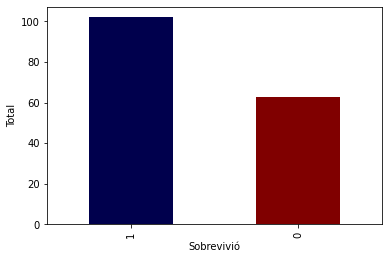
\includegraphics[width = 0.35\textwidth]{./sobrevivio.png}
\caption{\footnotesize \label{fig:sobrevivio}Cantidad de pacientes sobrevivientes y fallecidos del dataset}
\end{figure}
En el conjunto de datos se tienen variables de tipo categórico binario, ordinal, y númericas, se analizaron todos estos tipos de datos y a continuación se presentaran los resultados más relevantes.

\begin{figure}
\centering
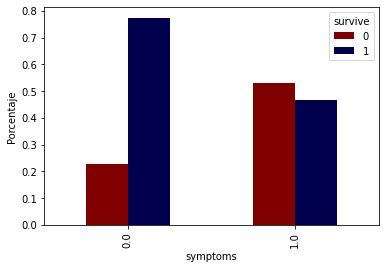
\includegraphics[width = 0.35\textwidth]{./sintomas.png}
\caption{\footnotesize \label{fig:synt}Porcentajes de fallecimientos para pacientes con y  sin  registro de síntomas}
\end{figure}


\subsection{Datos Categóricos Binarios}
\begin{figure}
\centering
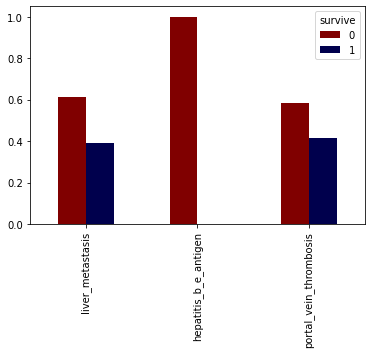
\includegraphics[width = 0.35\textwidth]{./nominal.png}
\caption{\footnotesize \label{fig:nom}Porcentajes de fallecimientos para hepatitis B, trombósis y pacientes con metástasis}
\end{figure}
Analizando los datos de este tipo se puede observar que de aquellos pacientes que no presentan síntomas (figura \ref{fig:synt}), casi el $80\%$ sobrevive,  lo que significa que el $20\%$ de aquellos que no se les registró ningún síntoma falleció. Es  importante destacar esto, debido a que el objetivo de este análisis es el de construir un modelo que aún sin el registro de síntomas en el paciente se pueda predecir si un paciente puede o no fallecer y tomar las medidas necesarias cuando corresponda y es que la falta de síntomas puede dar por hecho la salud del atendido, en la gráfica queda claro, que esto no debe ser así.
Por otro lado, en la figura \ref{fig:nom} se pueden observar las tres variables categóricas binarias que presentan un mayor porcentaje de fallecidos respecto al porcentaje de pacientes sobrevivientes. El $100\%$ de los pacientes a los que se les detecto el antígeno de la hepátitis B fallecieron, mientras que el $60\%$ tanto de los pacientes con trombósis y como de aquellos que presentan metástasis no sobrevivieron.


\subsection{Variables Ordinales}
En este caso el conjuto de datos cuenta solamente con tres variables ordinales, el \textit{performance status} que cuenta con cinco niveles, siguiendo la escala ECOG \cite{ECOG}. De manera ascendente nos indica el nivel de riesgo en que se encuentra el paciente de fallecer de acuerdo a las observaciones hechas por el personal de enfermería. Lo que se observa de los datos, es algo que se espera de acuerdo a lo ya dicho, entre mayor sea el  nivel de esta variable, hay un mayor porcentaje de muertes. La segunda variable ordinal es el grado de encefalopatía, esta cuenta con tres niveles: el primero cuando el sujeto presenta transtornos del sueño, letargo, apatía, cambios de personalidad, depresión o ansiedad. El segundo cuando el paciente tiene somnolencia, confusión desorientación o amnesia. Mientras que el tercero se asigna a aquellos pacientes en coma. Todo esto de acuerdo a la escala West Haven \cite{enc}. Es interesante observar el gráfico para esta variable (figura \ref{fig:ence}) puesto que el $100\%$ de los pacientes  en coma en este registro fallecieron. La última variable ordinal, es la ascitis. Esta es la acumulación anormal de líquido en el abdomen y tiene tres niveles de clasificación \cite{ascites}: uno, si solo es visible mediante una ecografía, dos, si es detectable con técnicas de palpamiento y tres, si es directamente visible. En la figura \ref{fig:ascites} se puede observar que de aquellos pacientes con grado 3 de ascitis, cerca del $70\%$ fallece.


\begin{figure}
\centering
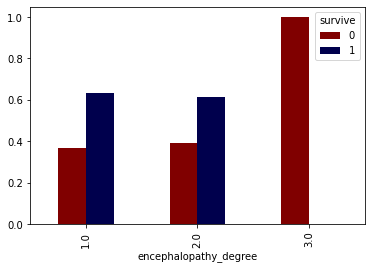
\includegraphics[width = 0.35\textwidth]{./ence.png}
\caption{\footnotesize \label{fig:ence}Porcentajes de fallecimientos para los distintos grados de encefalopatía.}
\end{figure}

\begin{figure}
\centering
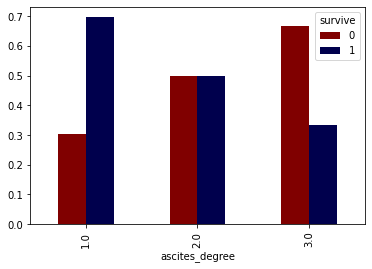
\includegraphics[width = 0.35\textwidth]{./ascites.png}
\caption{\footnotesize \label{fig:ascites}Porcentajes de fallecimientos para los distintos grados de ascitis.}
\end{figure}

\subsection{Variables Numéricas}

\begin{figure}
\centering
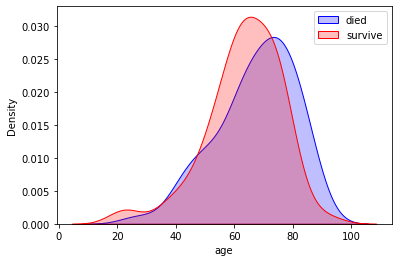
\includegraphics[width = 0.3\textwidth]{./age.png}
\caption{\footnotesize \label{fig:age}Distribución de fallecimientos y sobrevivientes de acuerdo a la edad.}
\end{figure}


En la figura \ref{fig:age} se puede distinguir que la cantidad de pacientes fallecidos es mayor a partir de los $65$ a\~nos, mientras que los menores a esa edad tienden a sobrevivir. Por otro lado, en la figura \ref{fig:hemo} se puede observar que para cantidades menores a los $13g/dL$ de hemoglobina los pacientes tienden a fallecer. Así mismo, estos datos indican que registrar niveles por debajo de los $4 g/dL$ de albumina podría poner la vida de un paciente en riesgo. Mientras que los niveles aceptables en el conteo de plaquetas deben ser menores a $450,000$. Por último, personas que presentan nódulos con una dimensión menor a los $7cm$ tienden a sobrevivir. De hecho clasificando el tama\~no de los nódulos en pequeños o grandes de a cuerdo a si estos son menores o mayores a $7cm$ se encontró que de aquellos que presentaron metástasis, cerca del $80\%$ registraron un nódulo con un tamaño mayor que $7cm$ por lo que esto podría ser un indicativo de la posibilidad de fallecimiento (figura \ref{fig:metnod}).

\begin{figure}
\centering
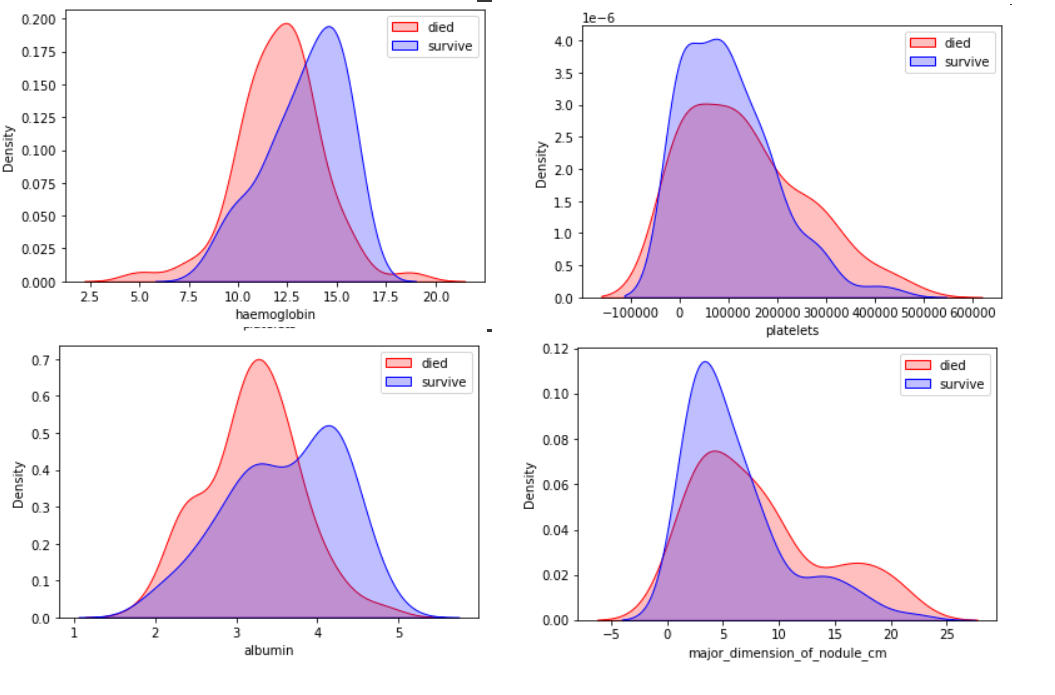
\includegraphics[width = 0.35\textwidth]{./hemo.png}
\caption{\footnotesize \label{fig:hemo}Distribución de fallecimientos y sobrevivientes de acuerdo al nivel de hemoglobina, el conteo de plaquetas, la albumina y el tama\~no de los nódulos linfáticos.}
\end{figure}

\begin{figure}
\centering
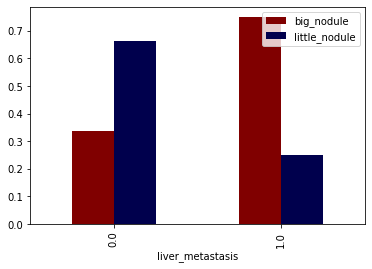
\includegraphics[width = 0.35\textwidth]{./met_nod.png}
\caption{\footnotesize \label{fig:metnod}Relación entre el tama\~no del nódulo y el registro de metástasis.}
\end{figure}

\section{Limpieza de Datos}
Los datos analizados son un registro llevado a cabo por personal médico, quienes decidieron llenar la información faltante con un signo de interrogación, por lo cual los valores nulos están representados con este símbolo. El dataset cuenta con una gran cantidad de valores faltantes. De hecho, variables como la saturación de oxígeno, ferritin e iron, presentan $48\%$ de valores nulos. En este caso se optó por eliminar columnas con un porcentaje de valores nulos mayor al $30\%$. \\
En el caso de las variables categóricas binarias y ordinales se sustituyeron los registros vacios con la moda de la columna en cuestión, mientras que en el caso de las variables númericas, se utilizó el algortimo de los \textit{K vecinos más cercanos} con la métrica Euclideana y un número de vecinos igual a $3$ para imputar los valores faltantes. 

\section{Preparación de los Datos}
Se crearon variables nuevas que clasifican al paciente en alguna categoría relacionada con el efecto observado de la variable númerica original en la posibilidad de supervivencia. Por ejemplo en casos como el ya mencionado, de la variable que contiene información del tama\~no del nódulo, se crearon dos categorias de acuerdo al tamaño, pequeño o grande, puesto que esto nos indica que el nodulo sea o no propenso a la metastasis y con ello que el  paciente sea propenso a morir. Lo que se hizo fué, aplicar la tecnica de bining para reducir el ruido de las variables númericas. Esto se realizó en las variables donde la gráfica de densidades indicaba una tendencia a fallecer o sobrevivir a partir de cierto límite. Las cuatro variables númericas analizadas en la sección anterior fueron procesadas bajo este esquema, entre otras.\\
Por último, se  transformaron todas las variables catégoricas, tanto las originales (variables ordinales) como las creadas mediante el proceso de bining a variables \textit{ dummies }. Toda esta limpieza y transformación de los datos nos dejó con un dataset que contiene $76$ variables, más la variable objetivo. El número de columnas se redujó posteriormente mediante la selección cíclica de variables.

\section{Modelado}
El objetivo del modelo es predecir si, con las características registradas de cada paciente, este sobreviviría o fallecería, por lo que el objetivo es claramente la creación de un clasficador binario, donde la variable target es \textit{survive}. Como se pudo observar en la figura \ref{fig:sobrevivio} el dataset está desbalanceado, por lo que se aplico el algoritmo \textit{SMOTE} de oversampling para balancearlo. Una vez hecho esto y con el conjunto balanceado, se dividió el conjunto en dos: el conjunto de entrenamiento y el conjunto de pruebas. Teniendo este último un tama\~no del $30\%$ del conjunto entero. También se probaronn dos tipos de transformación sobre los datos, la estandarización (\textit{StandardScaler}) y la normalización (\textit{MinMaxScaler}) debido a que los rangos de las columnas eran bastante variables, en particular podríamos mencionar la columna \textit{platalets} con valores del orden de cien mil, mientras que otras como la edad oscila entre los $20$ y $93$ a\~nos.\\
Se tiene una cantidad total de 76 variables que pueden ser posibles predictoras, por lo que fué necesario reducir el número de estas. Esto se realizó con una selección de características iterativa con ayuda del algoritmo \textit{RandomForesClassifier} donde el parámetro $n\_features\_to\_select$ fué variado entre $30$ y $60$ para encontrar el óptimo. El mínimo de este rango nos asegura tener la suficiente información para realizar las predicciones y el máximo asegura que se eliminen las posibles redundancias que existen sobre todo en las variables creadas. Además considerar este rango de iteraciones asegura que el entrenamiento de los modelos no sea tan costoso en cuestión de tiempo. \\
Con todo esto hecho, lo siguiente fué utilizar \textit{GridSearchCV} con un cv de $5$, esto dado que el número de registros es peque\~no. Se iteró sobre los siguientes algoritmos:
\begin{itemize}
\item \textit{LogisticRegression} variando el parámetro $C$ sobre los valores $0.0001, 0.001, 0.01, 0.1$ y $14$.
\item \textit{KNeighborsClassifier} variando el número de vecinos sobre $2, 3, 5, 7$ y $9$, el parámetro $p$ sobre $1, 2$ y para \textit{algorithm} se considerararon \textit{auto, $ball\_tree$, $kd\_tree$, brute}.
\item \textit{SVC}, variando el parámetro $C$ sobre los valores $0.001, 0.01, 0.1, 1, 10$ y $100$, el parámetro $gamma$ entre $0.05, 0.06, 0.07, 0.08, 0.09, 0.1, 0.2, 0.3, 0.4, 0.5$ y $0.6$ y se consideraron los \textit{kernels} siguientes: \textit{linear, rbf, poly, sigmoid}.
\item \textit{GaussianNB}
\item \textit{RandomForestClassifier}, variando los parámetros \textit{$n_estimators$} entre $10, 20, 100$ y $200$, \textit{$min\_samples\_leaf$} entre $1, 2, 4, 8$ y $10$, \textit{$max\_depth$} entre $2, 4, 6$ y $10$ y se consideró \textit{criterion} como \textit{entropy} y \textit{gini}, en cualquier caso se utilizó el parámetro \textit{$oob\_score$} como \textit{True}.
\item \textit{GradientBoostingClassifier}, variando los parámetros \textit{$max\_depth$} entre $2,4,6, 10, 20$ y $50$, \textit{$min\_samples\_leaf$} entre $1, 2, 4, 8$ y $10$, \textit{$n\_estimators$} entre $10, 20, 100$ y $200$, \textit{$learning\_rate$} entre $0.0001, 0.001, 0.01, 0.1$ y $1$, y por último, el parámetro \textit{loss} se consideró como \textit{deviance} y \textit{exponential}.
\end{itemize}
Para todos los casos se obtuvo el \textit{$accuracy\_score$}, \textit{$f1\_score$}, \textit{$precision\_score$} y \textit{$recall\_score$} así como la matriz de confusión.

\subsection{Modelo Ganador}
Dado el contexto del problema, cabe mencionar que es importante reducir al máximo el número de falsos positivos para poder detectar la mayor cantidad de pacientes con posibilidades de fallecer. Sin embargo, también resulta importante dismimnuir el número de falsos negativos, dado que al predecir la posibilidad de fallecimiento de un paciente, se invertirán recursos medicos y económicos en este cuando en realidad no los requiere con urgencia. Es por estas razones que se consideró la métrica \textit{f1} para elegir a los mejores algoritmos y posteriormente se priorizó el \textit{$precision\_score$} sin dejar de lado el \textit{$recall\_score$}. Con todo esto, el algoritmo seleccionado fué \textit{Support Vector Machine} para clasificación (\textit{SVC}) con los parámetros $C = 10$, $gamma = 0.5$ y con un \textit{kernel} \textit{rbf}. Cabe mencionar que el número de variables seleccionadas que resultó óptimo fué de $40$ y el transformador resultó ser \textit{MinMaxScaler}. Se obtuvieron las siguientes métricas para este algoritmo: $accuracy\_score = 0.91, f1\_score = 0.92, precision\_score = 0.88, recall\_score = 0.96$, con un número de falsos positivos de $5$ y un número de falsos negativos de $1$. Para disminuir la cantidad de falsos positivos se ajusto el threshold a $0.6$ con lo que se obtuvieron las siguientes métricas
\begin{itemize}
\item accuracy\_score = $0.90$
\item f1\_score = $0.90$
\item precision\_score = $0.93$
\item recall\_score = $0.87$
\end{itemize}

\subsection{Evaluación del Modelo}
\begin{figure}
\centering
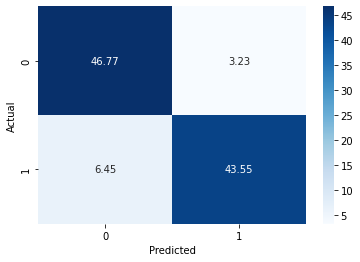
\includegraphics[width = 0.3\textwidth]{./matriz.png}
\caption{\footnotesize \footnotesize \label{fig:matriz}.Matriz de confusión SVC($C = 10$, $gamma = 0.5$, \textit{kernel} = \textit{rbf}), $\textit{threshold} = 0.6$,  $n\_features = 40$ y transformando los datos con \textit{MinMaxScaler}}
\end{figure}

En la matriz de confusión (figura \ref{fig:matriz}), se puede observar que se obtuvo un $4\%$ tanto de falsos positivos y como de  falsos negativos, esto corresponde a $3$ pacientes, en cada caso. \\ 
En la figura \ref{fig:pr} se puede apreciar la curva \textit{precision-recall}, de ella se puede ver que el modelo obtenido en este trabajo se encuentra en un buen punto de equilirbio entre la \textit{precisión} y el \textit{recall}, lo que se refleja en el \textit{f1 score} que resultó ser de $0.90$. \\
Por otro lado la curva \textit{ROC} se puede apreciar en la figura \ref{fig:lear}, se puede observar que es una curva bastante cargada hacia la esquina superior izquierda, por lo cual el modelo obtenido es un clasificador que aún teniendo un recall considerablemente alto, mantiene la tasa de falsos positivos baja, esto se comprueba al obtener la \textit{AUC}, que fué de  $0.95$. 
\begin{figure}
\centering
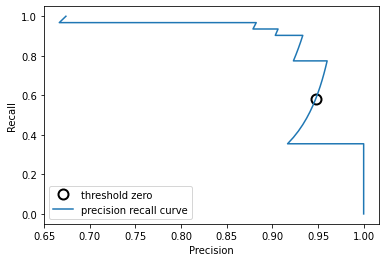
\includegraphics[width = 0.35\textwidth]{./precision_recall.png}
\caption{\footnotesize \label{fig:pr}.Precision-Recall  SVC($C = 10$, $gamma = 0.5$, \textit{kernel} = \textit{rbf}), $\textit{threshold} = 0.6$, $n\_features = 40$ y transformando los datos con \textit{MinMaxScaler}}
\end{figure}

\begin{figure}
\centering
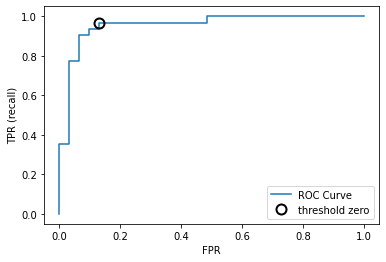
\includegraphics[width = 0.35\textwidth]{./ROC.png}
\caption{\footnotesize \label{fig:lear}.Curva ROC SVC($C = 10$, $gamma = 0.5$, \textit{kernel} = \textit{rbf}), $\textit{threshold} = 0.6$, $n\_features = 40$ y transformando los datos con \textit{MinMaxScaler}}
\end{figure}

Se hizo un modelo con \textit{cross-validation} utilizando \textit{stratified k-fold CV} de donde se obtuvieron las siguientes métricas:
\begin{itemize}
\item accuracy\_score = $0.82 \pm 0.11$
\item f1\_score = $0.83 \pm 0.11$
\item precision\_score = $0.85 \pm 0.14$
\item recall\_score = $0.82 \pm 0.14$
\end{itemize}

\subsection{Explicación del Modelo}
En la figura \ref{fig:shap} podemos apreciar un \textit{summary plot} de las variables que tienen más peso en las predicciones de la variable target. En esta se puede apreciar que la variable categ\'orica creada para la edad tiene un alto impacto en la predicción sobre el fallecimiento del paciente, como se mencionó antes, si el paciente es joven la posibilidad de sobrevivir aumenta drásticamente. Así mismo se puede notar que tanto si el paciente presenta ascetis de grado 1 como si se registra un alto nivel dehemoglobina, la posibilidad de sobrevivir aumenta. Por el contrario si presenta una cantidad pequeña de hemoglobina las posibilidades de fallecer aumentan. Algo similar sucede con la albumina. Por otro lado si el paciente presenta un performance status nivel 0 las posibilidades de sobrevivir son altas, lo que es congruente con el hecho de que es el nivel menos peligroso en la escala ECOG. Además si el paciente presenta sintomas esto tiene un mayor impacto en la posibilidad de fallecer. Si se observa la variable que indica si el tamaño del nódulo es pequeño se puede notar que, efectivamente entre menor sea su tamaño esto tiene un mayor impacto en predecir la supervivencia. Así mismo si el paciente presenta metastasis, esto influye en la predicción del fallecimiento del paciente. 
Cabe mencionar que la mayoría de las variables que influyen en las predicciones son las variables categóricas creadas a partir de las variables númericas.

\section{Análisis y Discusión de Resultados}
En este caso se buscó obtener un modelo que redujera al máximo la cantidad de falsos positivos, dado que es importante que no se de por superviviente a un paciente con una alta probabilidad de fallecer, por lo cual fué importante aumentar en la medida de lo posible la \textit{precisión}, en el trabajo presente se obtuvo una precisión del $85\%$ lo cual significa que de $100$ pacientes predichos como supervivientes, $15$ en realidad tienen una alta probabilidad de fallecer. En segundo lugar resultó también de importancia reducir el número de falsos negativos, puesto que al predecir que un paciente fallecerá se redirigirían recursos económicos y hospitalarios para salvaguardar la vida del paciente, cuando quisá no los requiera tanto como alguien en situación de emergencia o con altas probabilidades de morir, por ello se buscó optimizar el \textit{recall}. En el modelo obtenido en este trabajo, el recall resultó de $82\%$ lo que significa que de $100$ pacientes con posibilidades reales de ser supervivientes, $18$ serán predichos como pacientes que fallecerán. Sin duda alguna es un modelo con posibilidades de mejora, se puede, por ejemplo mejorar la colecta de datos para disminuir la cantidad de datos nulos y considerar en el modelo las variables eliminadas en este trabajo, por ejemplo los gramos de alcohol por a\~no, que sin duda tendría un impacto en la mejora de las métricas, puesto que la cirrosis es uno de los factores de riesgo para el HCC. Es importante prestar atención a las variables que resultaron ser de peso para las predicciones, como lo son la edad, la hemoglobina, el registro de hepatitis, etc. para la mejora en las predicciones.

\section{Conclusiones}
Este es un modelo que de implementarse ayudaría en la labor de los médicos de salvar vidas. Pues de $100$ pacientes con posibilidades reales de fallecer debido al HCC, al rededor de $85$, son personas de las cuales podría predecirse su situación con antelación y tomar las medidas necesarias para salvar su vida. Para aumentar este número se sugiere una mejora en la colecta de datos, y prestar especial atención a las variables mencionadas en la sección 6 que tienen un alto impacto en el destino del paciente que padece esta enfermedad. De estas variables aquellas que influyen positivamente en la posibilidad de fallecimiento, podría realizarse un estudio más profundo para llevar a cabo políticas públicas que ayuden a evitarlas, por ejemplo, acrecentar campañas contra el consumo de alcohol, agente preponderante en el desarrolo de la hepatitis y como se observó, por consecuencia en el desarrollo de HCC. Esto a la larga, podría traer el beneficio de disminuir la cantidad de pacientes de los que se sospeche padezcan esta terrible enfermedad.

\begin{figure}
\centering
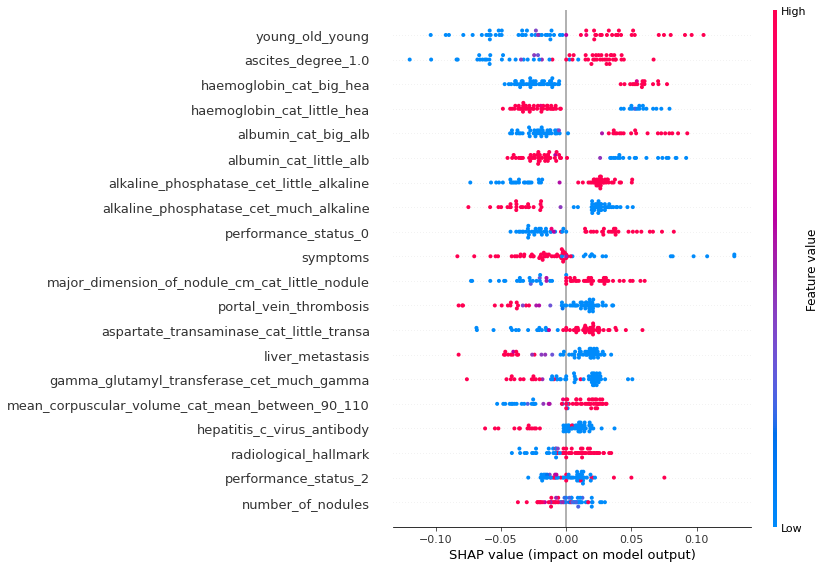
\includegraphics[width = 0.4\textwidth]{./exp.png}
\caption{\footnotesize \label{fig:shap}.Summary plot del modelo}
\end{figure}

\footnotesize
\begin{thebibliography}{0}

\bibitem{dataset} Datos obtenidos de: https://www.kaggle.com/datasets/mirlei/hcc-survival-data-set

\bibitem{HCC} Forner A, Reig M, Varela M,et al. Diagnosis and treatment of hepatocellular carcinoma. Update consensus document from the AEEH, SEOM, SERAM, SERVEI and SETH. Med Clin (Barc). 2016;146(11):511.e1-511.e22.

  \bibitem{ECOG} Oken, M.M., Creech, R.H., Tormey, D.C., Horton, J., Davis, T.E., McFadden, E.T., Carbone, P.P.: Toxicity And Response Criteria Of The Eastern Cooperative Oncology Group. Am J Clin Oncol 5:649-655, 1982.

\bibitem{enc}  Gutiérrez VI, Domínguez MA. Avances en los mecanismos fisiopatogénicos de la encefalopatía hepática. Rev Hosp M Gea Glz 2000; 3 (2): 60-70.

\bibitem{ascites} Moore, K. P.; Wong, F.; Gines, P.; Bernardi, M.; Ochs, A.; Salerno, F.; Angeli, P.; Porayko, M.; Moreau, R.; Garcia-Tsao, G.; Jimenez, W.; Planas, R.; Arroyo, V (2003). "The Management of Ascites in Cirrhosis: Report on the Consensus Conference of the International Ascites Club". Hepatology. 38 (1): 258–66.
\end{thebibliography}



\end{document}